\documentclass{article}

% Font
\usepackage[T1]{fontenc}
\usepackage[utf8]{inputenc}
\usepackage{lmodern}

% For tables
\usepackage{multirow}

% For identing the table at the right place
\usepackage{float}

% For left spacing
\usepackage{scrextend}

% For images
\usepackage{graphicx}

% for shorter paragraph spaces
\setlength{\parindent}{1ex}
\setlength{\parskip}{0.5ex}
% for first paragraphs
\newcommand*\fpar{\hspace{1ex}}

\title{Project 1 Requirements}
\author{Group 14 \\
Tiago Carvalho fc51034 \\
Diogo Lopes fc51058 \\
João Roque fc51080 \\
Miguel Saldanha fc51072 \\
João Afonso fc51111 \\
}
\date{03/03/2021}

\begin{document}
\maketitle

\section{Use Cases}
  \begin{table}[H]
    \centering
    \begin{tabular}{c|l} 
      User & Functionalities \\ \hline
      \multirow{5}{*}{ Regular } 
        & User Log in/Sign in \\
        & See Book, Show and Movie Library \\
        & Set Book/Show/Movie as seen \\
        & Set Book/Show/Movie as liked \\ 
        & Ask for sugestions to read and/or watch  \\ \hline
      \multirow{2}{*}{ Admin } 
        & Add Book/Show/Movie to Library \\
        & Remove Book/Show/Movie from Library
    \end{tabular}
  \end{table}

\section{Preliminary Functional and Non-Functional Requirements}
  
  \subsection{Functional}
    \begin{itemize}
      \item User should be able to browse Books, Shows and Movies
      \item User should be able to search for a specific item by name, type and/or categories
      \item User should be able to mark an Item as seen 
      \item User should be able to mark an Item as liked
      \item User should be able to ask for suggestions
      \item Admin should be able to add and remove content from the library
    \end{itemize}

  \subsection{Non-Functional}
    \begin{itemize}
      \item Browsing Items shouldn't take more than $1.5$ seconds to load
      \item Searching shouldn't take more than $2.5$ seconds loading the response
      \item Marking Item as seen or liked shouldn't take loading time on Users' end
      \item Suggestions shouldn't take more than $5$ seconds
      \item Data stored in cache shouldn't affect the system
      \item Adding and Removing Items should persist on the database
    \end{itemize}

\section{Preliminary Architectural Design}
  \begin{figure}[H]
    \centering
    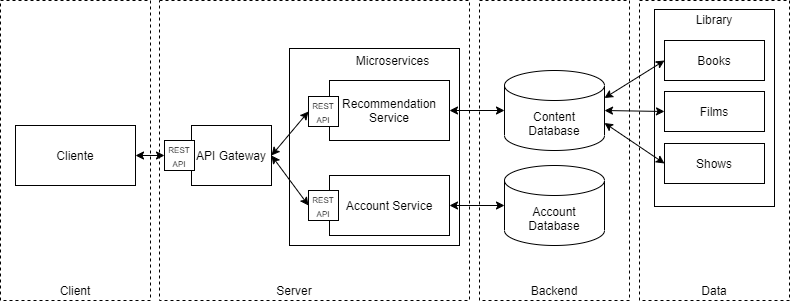
\includegraphics[width=\textwidth]{"images/CloudNativeAppArchitectureV1.png"}
  \end{figure}

\end{document}